% ============================================================
%  FedQPSO vs FedAvg — IEEE Conference Paper
%  Author: Divyansh Teja Edla
%  Matrusri Engineering College, Hyderabad, India
% ============================================================
\documentclass[conference]{IEEEtran}
\IEEEoverridecommandlockouts

\usepackage{cite}
\usepackage{amsmath,amssymb,amsfonts}
\usepackage{algorithmic}
\usepackage{algorithm}
\usepackage{graphicx}
\usepackage{textcomp}
\usepackage{xcolor}
\usepackage{booktabs}
\usepackage{multirow}
\usepackage{array}
\usepackage{url}
\usepackage{hyperref}

\graphicspath{{figs/}}

\def\BibTeX{{\rm B\kern-.05em{\sc i\kern-.025em b}\kern-.08em
    T\kern-.1667em\lower.7ex\hbox{E}\kern-.125emX}}

% ============================================================
\begin{document}
% ============================================================

\title{FedQPSO: Overcoming FedAvg Inequity in Non-IID Federated Brain
Tumor Classification via Layer-by-Layer Quantum Particle Swarm Optimization
\thanks{This work was supported by the Department of Computer Science \&
Engineering, Matrusri Engineering College, Hyderabad, India.}}

\author{%
\IEEEauthorblockN{Divyansh Teja Edla}
\IEEEauthorblockA{\textit{Dept.\ of Computer Science \& Engineering}\\
\textit{Matrusri Engineering College}\\
Hyderabad, India\\
divyanshteja.edla@gmail.com}
}

\maketitle

% ============================================================
\begin{abstract}
Federated Averaging (FedAvg), the dominant aggregation algorithm in
Federated Learning (FL), produces globally high accuracy that systematically
conceals severe per-institution performance disparities under Non-IID data —
a critical failure mode in multi-hospital medical imaging deployments. We
propose \textbf{FedQPSO}, a server-side aggregation algorithm that replaces
FedAvg's weighted mean with a layer-by-layer Quantum Particle Swarm
Optimization (QPSO) search guided by combined cross-client validation loss.
This fitness-driven mechanism acts as an implicit fairness constraint,
converging toward weights that minimize loss simultaneously across all
clients without any explicit fairness regularizer. We evaluate FedQPSO
against FedAvg on four-class brain tumor MRI classification across three
heterogeneous clinical sites under natural heterogeneity (Setup~1) and
moderate label skew 70/10/10/10 (Setup~2). FedQPSO reduces the inter-client
accuracy gap by \textbf{81\%} in Setup~1 and \textbf{72\%} in Setup~2
relative to FedAvg, is the only method maintaining $\geq$80\% accuracy at
the weakest client under label skew (80.00\% vs.\ 60.42\% for FedAvg), and
achieves the highest Glioma recall in both setups (0.9593; 0.8914). FedQPSO
is the only method statistically significantly outperforming FedAvg under
natural heterogeneity ($p = 0.000882$, Cohen's $d = 0.35$), with effect size
scaling to $d = 1.26$ under label skew — confirming the algorithm is most
advantageous precisely when data conditions are most challenging.
\end{abstract}

\begin{IEEEkeywords}
Federated learning, FedQPSO, FedAvg, quantum particle swarm optimization,
brain tumor classification, non-IID data, client fairness, medical imaging, MRI
\end{IEEEkeywords}

% ============================================================
\section{Introduction}
\label{sec:intro}
% ============================================================

Brain tumors carry a five-year survival rate under 36\% for malignant cases
\cite{ostrom2021}. Accurate MRI-based classification — distinguishing gliomas,
meningiomas, pituitary adenomas, and healthy tissue — is fundamental to
treatment planning. Deep learning models achieve near-expert performance when
trained on large, diverse datasets \cite{sultan2019}, but assembling such
datasets across institutions is blocked by strict data privacy regulations:
HIPAA in the United States \cite{hipaa}, GDPR in the European Union, and
comparable frameworks globally prohibit sharing raw patient records.

\textbf{Federated Learning (FL)} \cite{mcmahan2017} circumvents this by
decoupling model training from data centralization: each hospital trains
locally on its private data, and only model weight updates — never raw images
— are transmitted to a central server for aggregation. This approach has
shown strong results in brain tumor segmentation \cite{sheller2018} and
broader medical imaging applications \cite{rieke2020}.

The standard aggregation algorithm, \textbf{FedAvg} \cite{mcmahan2017},
computes a dataset-size-weighted average of client weights. Under real-world
\textbf{Non-IID} conditions — where hospitals differ in scanner equipment,
patient demographics, and class distributions — this weighted average is
dominated by large clients. The result: a global model that achieves high
\emph{average} accuracy while systematically failing smaller or
class-imbalanced institutions \cite{zhao2018}. A model reporting 90\% global
accuracy with one hospital simultaneously at 52\% is not a success — it is a
fairness failure with direct patient safety implications.

This paper addresses this failure directly. We propose \textbf{FedQPSO}, a
novel server-side aggregation algorithm that replaces FedAvg's closed-form
weighted mean with an iterative, fitness-guided Quantum Particle Swarm
Optimization (QPSO) \cite{sun2004qpso} search, applied \emph{layer-by-layer}
over the global model. The fitness function evaluates candidate weight
tensors against a combined cross-client validation set, naturally penalizing
solutions that perform well for large clients but fail small ones. No explicit
fairness objective is required — fairness emerges from the structure of
fitness evaluation itself.

\textbf{Key contributions:}
\begin{enumerate}
    \item \textbf{FedQPSO algorithm:} A novel federated aggregation method
    performing layer-by-layer QPSO with validation-loss fitness evaluation at
    the server side, with no change to client-side training.

    \item \textbf{Empirical fairness demonstration:} Formal comparison
    showing FedQPSO reduces FedAvg's max-min per-client accuracy gap by
    72--81\% across two real-world Non-IID conditions.

    \item \textbf{Clinical equity:} FedQPSO is the only method maintaining
    $\geq$80\% accuracy at the weakest client under label skew, with the
    highest Glioma recall in both experimental conditions.

    \item \textbf{Statistical validation:} Paired $t$-tests confirm FedQPSO
    statistically significantly outperforms FedAvg under both natural
    heterogeneity ($p = 0.000882$) and label skew ($p = 2.91\times10^{-22}$),
    with Cohen's $d$ scaling from 0.35 to 1.26 as heterogeneity increases.

    \item \textbf{Stability:} FedQPSO exhibits the lowest accuracy
    volatility across all 200 training rounds — maximum single-round drop
    of 3.38\,pp versus 14.78\,pp for FedAvg.
\end{enumerate}

% ============================================================
\section{Related Work}
\label{sec:related}
% ============================================================

\subsection{Federated Learning for Medical Imaging}
McMahan et al.\ \cite{mcmahan2017} introduced FedAvg in 2017. Sheller et al.\
\cite{sheller2018} demonstrated FL for brain tumor segmentation on BraTS,
showing results approaching centralized training. Rieke et al.\
\cite{rieke2020} surveyed FL in healthcare, identifying Non-IID data as the
central unsolved challenge. These works establish the FL paradigm we extend,
but do not address per-client equity in classification settings.

\subsection{Non-IID Data and FedAvg Failures}
Zhao et al.\ \cite{zhao2018} analyzed how label skew degrades FedAvg
accuracy, quantifying divergence between local and global optima as the
primary mechanism. Li et al.\ \cite{li2021survey} surveyed FL challenges,
confirming that data heterogeneity is the primary barrier to deployment.
Our work demonstrates that the \emph{fairness} impact of FedAvg under
Non-IID conditions — not just global accuracy degradation — is the more
clinically consequential failure mode.

\subsection{PSO and QPSO in Machine Learning}
Classical PSO \cite{kennedy1995} has been applied to neural architecture
search and weight initialization. FedPSO \cite{fedpso2021} uses classical PSO
for FL global model updates, transmitting score values rather than weight
tensors to reduce communication. Sun et al.\ \cite{sun2004qpso} introduced
QPSO, extending PSO with quantum-inspired position updates for theoretically
proven global search capability. Our prior work \cite{edla2025mnist}
applied layerwise QPSO to FL aggregation on IID MNIST data (81.5\% vs.\
FedAvg's 41.2\%). The present paper is the first extension to Non-IID medical
imaging, with formal fairness analysis and clinical evaluation.

% ============================================================
\section{System Model and Problem Formulation}
\label{sec:problem}
% ============================================================

Let $\mathcal{K} = \{1, 2, \ldots, K\}$ be $K$ clients, each holding private
dataset $\mathcal{D}_k$ with $n_k$ samples, $N = \sum_k n_k$. The standard
FL objective is:
\begin{equation}
    \min_{w}\; F(w) = \sum_{k=1}^{K} \frac{n_k}{N}\, F_k(w),
    \label{eq:fl_objective}
\end{equation}
where $F_k(w) = \mathbb{E}_{(x,y)\sim\mathcal{D}_k}[\ell(w;\,x,y)]$. Under
Non-IID conditions, minimizing~\eqref{eq:fl_objective} yields solutions that
minimize average loss but leave minority clients' $F_k(w)$ poorly minimized.

We define an additional \textbf{fairness objective}:
\begin{equation}
    \min_{w}\; \sigma^2\!\left(F_1(w), F_2(w), \ldots, F_K(w)\right).
    \label{eq:fairness_objective}
\end{equation}
FedAvg pursues only~\eqref{eq:fl_objective}. FedQPSO jointly pursues
both objectives by evaluating candidate weights against a balanced
cross-client validation set, directly penalizing solutions that fail any
participating institution.

% ============================================================
\section{Methodology}
\label{sec:method}
% ============================================================

\subsection{FedAvg (Baseline)}
FedAvg \cite{mcmahan2017} aggregates by dataset-size-weighted mean:
\begin{equation}
    w^{(r+1)} = \sum_{k=1}^{K} \frac{n_k}{N}\, w_k^{(r)}.
    \label{eq:fedavg}
\end{equation}
This is deterministic, stateless, and computationally negligible. Under
Non-IID conditions, large clients dominate $w^{(r+1)}$, embedding their
local optima into the global model at the expense of minority institutions.
FedAvg has no mechanism to detect or correct this bias.

\subsection{FedQPSO: Proposed Algorithm}

\subsubsection{QPSO Background}
QPSO \cite{sun2004qpso} models each candidate solution as a particle in a
quantum potential well. Given personal best $\mathbf{pbest}_i$, global best
$\mathbf{gbest}$, and mean best $\mathbf{mbest}$, the position update is:
\begin{align}
    \phi &\sim \mathcal{U}(0,1), \quad
    p_i = \phi\,\mathbf{pbest}_i + (1-\phi)\,\mathbf{gbest},
    \label{eq:attractor}\\
    \mathbf{mbest} &= \frac{1}{K}\sum_{k=1}^{K}\mathbf{pbest}_k,
    \label{eq:mbest}\\
    x_i^{(t+1)} &= p_i \pm \beta\,|{\mathbf{mbest}} - x_i^{(t)}|
    \cdot \ln\!\left(\frac{1}{u}\right), \; u \sim \mathcal{U}(\varepsilon,1),
    \label{eq:qpso_update}
\end{align}
where sign ($\pm$) is chosen uniformly at random and $\beta$ is the
contraction-expansion coefficient. The logarithmic distribution enables
quantum tunneling — particles can escape local optima by jumping to distant
regions of the weight space.

\subsubsection{Layer-by-Layer Federated Aggregation}
\textbf{Why layer-by-layer?} A naive application of QPSO over the entire
weight tensor simultaneously (120K parameters) without fitness evaluation
is indistinguishable from noise injection. Phase~3 experiments with such
naive QPSO yielded 77.3\% global accuracy versus FedAvg's 90.56\% under
label skew. The layer-by-layer decomposition with per-layer fitness evaluation
transforms QPSO from a noise source into a disciplined optimization procedure.

At each round $r$, after all clients complete local training, FedQPSO
executes Algorithm~\ref{alg:fedqpso}.

\begin{algorithm}
\caption{FedQPSO server-side aggregation (round $r$)}
\label{alg:fedqpso}
\begin{algorithmic}[1]
\REQUIRE Client weights $\{w_k\}_{k=1}^K$; combined val set
$\mathcal{V} = \bigcup_k \mathcal{V}_k$; $\beta$, iterations $T$
\STATE Compute FedAvg baseline $\bar{w}$ \hfill\COMMENT{covers BatchNorm stats}
\FOR{each trainable layer $\ell = 1,\ldots,L$}
    \STATE Initialize particles: $x_k \leftarrow w_k[\ell]$ for all $k$
    \STATE Evaluate $\mathrm{fit}(x_k) \leftarrow \mathcal{L}(\bar{w}[x_k \to \ell],\;\mathcal{V})$
    \STATE $\mathbf{pbest}_k \leftarrow x_k$;\; $\mathbf{gbest} \leftarrow \arg\min_k \mathrm{fit}(x_k)$
    \FOR{$t = 1$ to $T$}
        \STATE Compute $\mathbf{mbest}$ via \eqref{eq:mbest}
        \FOR{each particle $k$}
            \STATE Compute $p_k$ via \eqref{eq:attractor}; sample $u, \phi$; choose $\pm$
            \STATE $x_k^{(t+1)} \leftarrow p_k \pm \beta|\mathbf{mbest}-x_k^{(t)}|\cdot\ln(1/u)$
            \STATE Evaluate $\mathrm{fit}(x_k^{(t+1)})$
            \IF{$\mathrm{fit}(x_k^{(t+1)}) < \mathrm{fit}(\mathbf{pbest}_k)$}
                \STATE $\mathbf{pbest}_k \leftarrow x_k^{(t+1)}$
            \ENDIF
            \IF{$\mathrm{fit}(x_k^{(t+1)}) < \mathrm{fit}(\mathbf{gbest})$}
                \STATE $\mathbf{gbest} \leftarrow x_k^{(t+1)}$
            \ENDIF
        \ENDFOR
    \ENDFOR
    \STATE $w^{(r+1)}[\ell] \leftarrow \mathbf{gbest}$ \hfill\COMMENT{commit best weights}
\ENDFOR
\RETURN assembled global model $w^{(r+1)}$
\end{algorithmic}
\end{algorithm}

\subsubsection{Implicit Fairness Mechanism}
The combined validation set $\mathcal{V}$ contains samples from all clients.
A weight configuration achieving low validation loss for large clients but
high loss for Client~1 produces high aggregate fitness and is rejected.
Iteratively, the QPSO search converges toward weights that satisfy both
objectives~\eqref{eq:fl_objective} and~\eqref{eq:fairness_objective}
simultaneously — without any fairness hyperparameter or explicit objective.

\subsubsection{Computational Cost}
Per round: $KL(1+T)$ forward passes. With $K=3$, $L=16$, $T=5$: $288$
forward passes per round, versus FedAvg's $O(1)$ averaging operation.
This concentrates the $9.4\times$ overhead exclusively at the central server;
client-side training cost is identical for both algorithms.

% ============================================================
\section{Experimental Setup}
\label{sec:setup}
% ============================================================

\subsection{Datasets and Client Configuration}
Two publicly available brain tumor MRI datasets partition into three
simulated hospital clients (Table~\ref{tab:clients}).

\begin{table}[htbp]
\caption{Dataset and Client Configuration}
\label{tab:clients}
\begin{center}
\begin{tabular}{lcccc}
\hline
\textbf{Client} & \textbf{Source} & \textbf{Train} & \textbf{Val} &
\textbf{Test}\\
\hline
Client 1 & Masoud MRI \cite{masoud} (test split)  & 1,119 & 240 & 241\\
Client 2 & BRISC 2025 \cite{brisc} (train split)  & 3,499 & 750 & 751\\
Client 3 & Masoud MRI \cite{masoud} (train split) & 3,919 & 840 & 841\\
\hline
\textbf{Global Test} & Combined & --- & --- & \textbf{1,833}\\
\hline
\multicolumn{5}{l}{\small Glioma: 442, Meningioma: 470, No Tumor: 432,
Pituitary: 489.}
\end{tabular}
\end{center}
\end{table}

Data never crosses client boundaries; Non-IID conditions are created by
subsampling within each client's own dataset, preserving FL privacy.
Client~1 holds $3.5\times$ fewer samples than Client~3, representing the
kind of institutional size imbalance typical of real-world hospital networks.

\subsection{Heterogeneity Conditions}

\textbf{Setup 1 --- Natural Heterogeneity:} Clients retain their native
class distributions from independent real-world source datasets.
Heterogeneity arises organically from scanner variation and slight
class imbalances, reflecting a realistic best-case deployment scenario.

\textbf{Setup 2 --- Moderate Label Skew (70/10/10/10):} Each client's
training data is restructured so 70\% belongs to one dominant class and 10\%
each to the remaining three — Client~1 $\to$ Glioma; Client~2 $\to$ Meningioma;
Client~3 $\to$ No Tumor. Minority-class images are augmented (horizontal flip,
rotation $\pm30^\circ$, brightness/contrast jitter, Gaussian blur) to fulfill
the target distribution. This represents a challenging Non-IID scenario
deliberately designed to expose FedAvg's weaknesses.

\subsection{Model Architecture}
All experiments use \textbf{SimpleCNN} ($\approx$155K parameters), chosen
deliberately lightweight to ensure aggregation algorithm is the primary
performance determinant, free from confounds introduced by model capacity or
pretrained features:

{\small\begin{verbatim}
3x112x112->Conv(3,16)->BN->ReLU->Pool
         ->Conv(16,32)->BN->ReLU->Pool
         ->Conv(32,64)->BN->ReLU->AAPool
         ->Dropout(0.3)->FC(1024,128)->ReLU
         ->Dropout(0.3)->FC(128,4)
Total: 155,524 params; 16 trainable tensors
\end{verbatim}}

\subsection{Hyperparameters}
Table~\ref{tab:hyperparams} lists all training hyperparameters. Early
stopping triggers when global accuracy reaches $\geq$95\% and fails to
improve for 15 consecutive rounds (minimum 30 rounds).

\begin{table}[htbp]
\caption{Training Hyperparameters}
\label{tab:hyperparams}
\begin{center}
\begin{tabular}{lc}
\hline
\textbf{Parameter} & \textbf{Value}\\
\hline
Max communication rounds         & 100\\
Local epochs per round           & 1\\
Local optimizer                  & Adam\\
Learning rate                    & 0.01\\
Batch size                       & 64\\
Image size                       & $112 \times 112$\\
FedQPSO $\beta$                  & 0.6 (static)\\
FedQPSO QPSO iterations $T$      & 5\\
Early stopping patience          & 15 rounds\\
Hardware                         & Tesla P100-16GB (Kaggle)\\
Framework                        & PyTorch 2.x, Python 3.12\\
Random seed                      & 42\\
\hline
\end{tabular}
\end{center}
\end{table}

\subsection{Evaluation Metrics}
\textbf{Primary:} Global test accuracy, per-class precision/recall/F1-score,
ROC-AUC (per-class and micro-average).
\textbf{Fairness:} Per-client validation accuracy standard deviation
($\sigma$) and max-minus-min gap at final round and best-round checkpoint.
\textbf{Stability:} Maximum single-round accuracy drop; round-to-round
accuracy standard deviation.
\textbf{Statistical:} Paired two-tailed $t$-test on per-round accuracy
sequences; Cohen's $d$ effect size.
\textbf{Convergence:} Rounds to first reach 80\% global accuracy.

% ============================================================
\section{Results}
\label{sec:results}
% ============================================================

\subsection{Global Accuracy}

Tables~\ref{tab:global_s1} and~\ref{tab:global_s2} compare FedAvg and
FedQPSO on global test accuracy.

\begin{table}[htbp]
\caption{Global Test Accuracy --- Setup 1 (Natural Heterogeneity)}
\label{tab:global_s1}
\begin{center}
\begin{tabular}{lcc}
\hline
\textbf{Metric} & \textbf{FedAvg} & \textbf{FedQPSO}\\
\hline
Best Accuracy (\%)    & 95.80\% (r83) & 95.14\% (r89)\\
Final Accuracy (\%)   & 93.29\% (r98) & 93.78\% (r100)\\
Rounds run            & 98$^\dagger$  & 100\\
Rounds to 80\%        & 11            & \textbf{9}\\
Avg.\ round time (s)  & 7.84          & 75.09\\
\hline
\multicolumn{3}{l}{\small $^\dagger$Early stopping ($\geq$95\%,
no improvement for 15 rounds).}
\end{tabular}
\end{center}
\end{table}

\begin{table}[htbp]
\caption{Global Test Accuracy --- Setup 2 (Moderate Label Skew)}
\label{tab:global_s2}
\begin{center}
\begin{tabular}{lcc}
\hline
\textbf{Metric} & \textbf{FedAvg} & \textbf{FedQPSO}\\
\hline
Best Accuracy (\%)    & 90.56\% (r94)  & \textbf{92.09\%} (r98)\\
Final Accuracy (\%)   & 88.16\% (r100) & \textbf{91.43\%} (r100)\\
Rounds to 80\%        & 35             & \textbf{19}\\
Avg.\ round time (s)  & 8.03           & 74.92\\
\hline
\end{tabular}
\end{center}
\end{table}

Under natural heterogeneity (Setup~1), both methods reach high global
accuracy ($>$93\%), with FedAvg marginally leading on peak accuracy (95.80\%
vs.\ 95.14\%). FedQPSO converges faster (9 vs.\ 11 rounds to 80\%) and
achieves a slightly higher \emph{final} accuracy (93.78\% vs.\ 93.29\%),
indicating it avoids the late-round degradation caused by early stopping
in FedAvg. Under label skew (Setup~2), FedQPSO clearly outperforms FedAvg
across every metric: best accuracy (+1.53\,pp), final accuracy (+3.27\,pp),
and convergence speed (19 vs.\ 35 rounds to 80\%). Critically, the global
accuracy gap understates FedQPSO's advantage — the full story is told by
per-client fairness metrics.



\subsection{Per-Class Classification Performance}

Table~\ref{tab:perclass} reports per-class F1-score and Glioma recall
at each method's best-round checkpoint.

\begin{table}[htbp]
\caption{Per-Class F1-Score and Glioma Recall at Best Checkpoint}
\label{tab:perclass}
\begin{center}
\renewcommand{\arraystretch}{1.15}
\begin{tabular}{llcc}
\hline
\textbf{Setup} & \textbf{Class} & \textbf{FedAvg} & \textbf{FedQPSO}\\
\hline
\multirow{5}{*}{S1 F1}
 & Glioma     & 0.9438 & \textbf{0.9560}\\
 & Meningioma & \textbf{0.9378} & 0.9211\\
 & No Tumor   & \textbf{0.9663} & 0.9602\\
 & Pituitary  & \textbf{0.9828} & 0.9686\\
 & Macro Avg  & \textbf{0.9577} & 0.9515\\
\hline
\multirow{5}{*}{S2 F1}
 & Glioma     & 0.8841 & \textbf{0.9089}\\
 & Meningioma & 0.8458 & \textbf{0.8727}\\
 & No Tumor   & 0.9447 & \textbf{0.9528}\\
 & Pituitary  & 0.9491 & \textbf{0.9507}\\
 & Macro Avg  & 0.9059 & \textbf{0.9213}\\
\hline
\multirow{2}{*}{Recall}
 & Glioma (S1) & 0.9118 & \textbf{0.9593}\\
 & Glioma (S2) & 0.8371 & \textbf{0.8914}\\
\hline
\end{tabular}
\end{center}
\end{table}

Under label skew (Setup~2), FedQPSO outperforms FedAvg on \emph{every}
class metric, including a 2.48\,pp Macro F1 improvement. Under natural
heterogeneity, FedAvg leads on Meningioma, No Tumor, and Pituitary F1,
while FedQPSO leads on the \textbf{most clinically critical class: Glioma},
in both setups. FedQPSO's Glioma recall improvement over FedAvg in
Setup~2 (5.43\,pp) translates to approximately \textbf{24 additional
correctly identified glioma cases per 1,000 patients} — a direct patient
safety benefit.

\subsection{Client Fairness}
\label{sec:fairness}

Table~\ref{tab:fairness} presents per-client performance metrics.

\begin{table}[htbp]
\caption{Client Fairness Metrics (Final Round and At-Peak-Round)}
\label{tab:fairness}
\begin{center}
\renewcommand{\arraystretch}{1.15}
\begin{tabular}{llcc}
\hline
\textbf{Setup} & \textbf{Metric} & \textbf{FedAvg} & \textbf{FedQPSO}\\
\hline
\multirow{4}{*}{S1}
 & Cl.\ 1 accuracy, final (\%)  & 83.75 & \textbf{92.08}\\
 & Client $\sigma$, final        & 5.28\% & \textbf{1.56\%}\\
 & Max$-$Min gap (pp)            & 12.20 & \textbf{2.32}\\
 & Client $\sigma$, at peak      & 9.50\% & \textbf{1.62\%}\\
\hline
\multirow{4}{*}{S2}
 & Cl.\ 1 accuracy, final (\%)  & 60.42 & \textbf{80.00}\\
 & Client $\sigma$, final        & 12.82\% & \textbf{3.65\%}\\
 & Max$-$Min gap (pp)            & 28.75 & \textbf{8.10}\\
 & Client $\sigma$, at peak      & 13.38\% & \textbf{4.23\%}\\
\hline
\end{tabular}
\end{center}
\end{table}



FedQPSO's fairness improvements are decisive:
\begin{itemize}
    \item \textbf{Setup 1:} Max-min gap reduced from 12.20\,pp to 2.32\,pp
    (\textbf{81\% reduction}); client $\sigma$ from 5.28\% to 1.56\%.
    Client~1 final accuracy improves by +8.33\,pp (83.75\% $\to$ 92.08\%).

    \item \textbf{Setup 2:} Max-min gap reduced from 28.75\,pp to 8.10\,pp
    (\textbf{72\% reduction}); client $\sigma$ from 12.82\% to 3.65\%.
    Client~1 final accuracy improves by +19.58\,pp (60.42\% $\to$ 80.00\%).
\end{itemize}

The most clinically stark comparison: at FedAvg's Setup~2 peak (90.56\%
global, r94), Client~1's concurrent validation accuracy was \textbf{52.92\%}
--- barely above chance. At FedQPSO's peak (92.09\%, r98), Client~1 was at
\textbf{80.83\%} --- a 27.91\,pp improvement for the weakest hospital at the
same moment of best global performance. Global accuracy alone would present
both models as broadly equivalent; client-level analysis reveals a profound
difference in real-world clinical utility.

\subsection{Statistical Significance}

Table~\ref{tab:stats} reports paired two-tailed $t$-tests on full per-round
global accuracy sequences.

\begin{table}[htbp]
\caption{Statistical Significance: Paired $t$-Test (FedAvg vs.\ FedQPSO)}
\label{tab:stats}
\begin{center}
\begin{tabular}{lcccl}
\hline
\textbf{Setup} & $t$ & $p$ & $d$ & \textbf{Significant?}\\
\hline
S1 (Natural Heterogeneity) & 3.43 & 0.000882 & 0.35 & Yes ($p < 0.001$)\\
S2 (Label Skew)            & 12.59 & $2.91\times10^{-22}$ & 1.26 & Yes ($p \ll 0.001$)\\
\hline
\multicolumn{5}{l}{\small $d$: Cohen's effect size. S2 uses 100 rounds for
both methods.}
\end{tabular}
\end{center}
\end{table}

FedQPSO statistically significantly outperforms FedAvg in \textbf{both}
experimental conditions. Under natural heterogeneity the effect is medium
($d = 0.35$, $p = 0.000882$); under label skew it becomes very large
($d = 1.26$, $p = 2.91\times10^{-22}$). This scaling of Cohen's $d$ from
0.35 to 1.26 as heterogeneity increases provides strong evidence that
\textbf{FedQPSO's advantage is most pronounced precisely when conditions are
most clinically challenging} — the exact scenario where algorithm choice
matters most.

\subsection{ROC-AUC Analysis}

Table~\ref{tab:auc} reports AUC values.

\begin{table}[htbp]
\caption{ROC-AUC Per Class and Micro-Average}
\label{tab:auc}
\begin{center}
\begin{tabular}{lcccc}
\hline
& \multicolumn{2}{c}{\textbf{Setup 1}} &
  \multicolumn{2}{c}{\textbf{Setup 2}}\\
\cmidrule(lr){2-3}\cmidrule(lr){4-5}
\textbf{Class} & \textbf{FedAvg} & \textbf{FedQPSO} &
                 \textbf{FedAvg} & \textbf{FedQPSO}\\
\hline
Glioma     & 0.988 & \textbf{0.991} & 0.977 & \textbf{0.985}\\
Meningioma & \textbf{0.992} & 0.986 & 0.970 & \textbf{0.978}\\
No Tumor   & \textbf{0.998} & 0.995 & 0.996 & \textbf{0.997}\\
Pituitary  & \textbf{0.999} & 0.998 & 0.996 & \textbf{0.997}\\
Micro Avg  & \textbf{0.995} & 0.993 & 0.986 & \textbf{0.990}\\
\hline
\end{tabular}
\end{center}
\end{table}

Both methods achieve clinically excellent AUC (no value below 0.970 in either
setup). FedQPSO leads \textbf{Glioma AUC in both setups} --- consistent with
its superior Glioma recall and F1 performance. Under label skew, FedQPSO
improves Glioma AUC by 0.008, Meningioma AUC by 0.008, and micro-average
AUC by 0.004 relative to FedAvg.



\subsection{Confusion Matrices}

Figs.~\ref{fig:cm_s1} and~\ref{fig:cm_s2} show confusion matrices at
best-round checkpoints.

\begin{figure}[htbp]
\centerline{%
  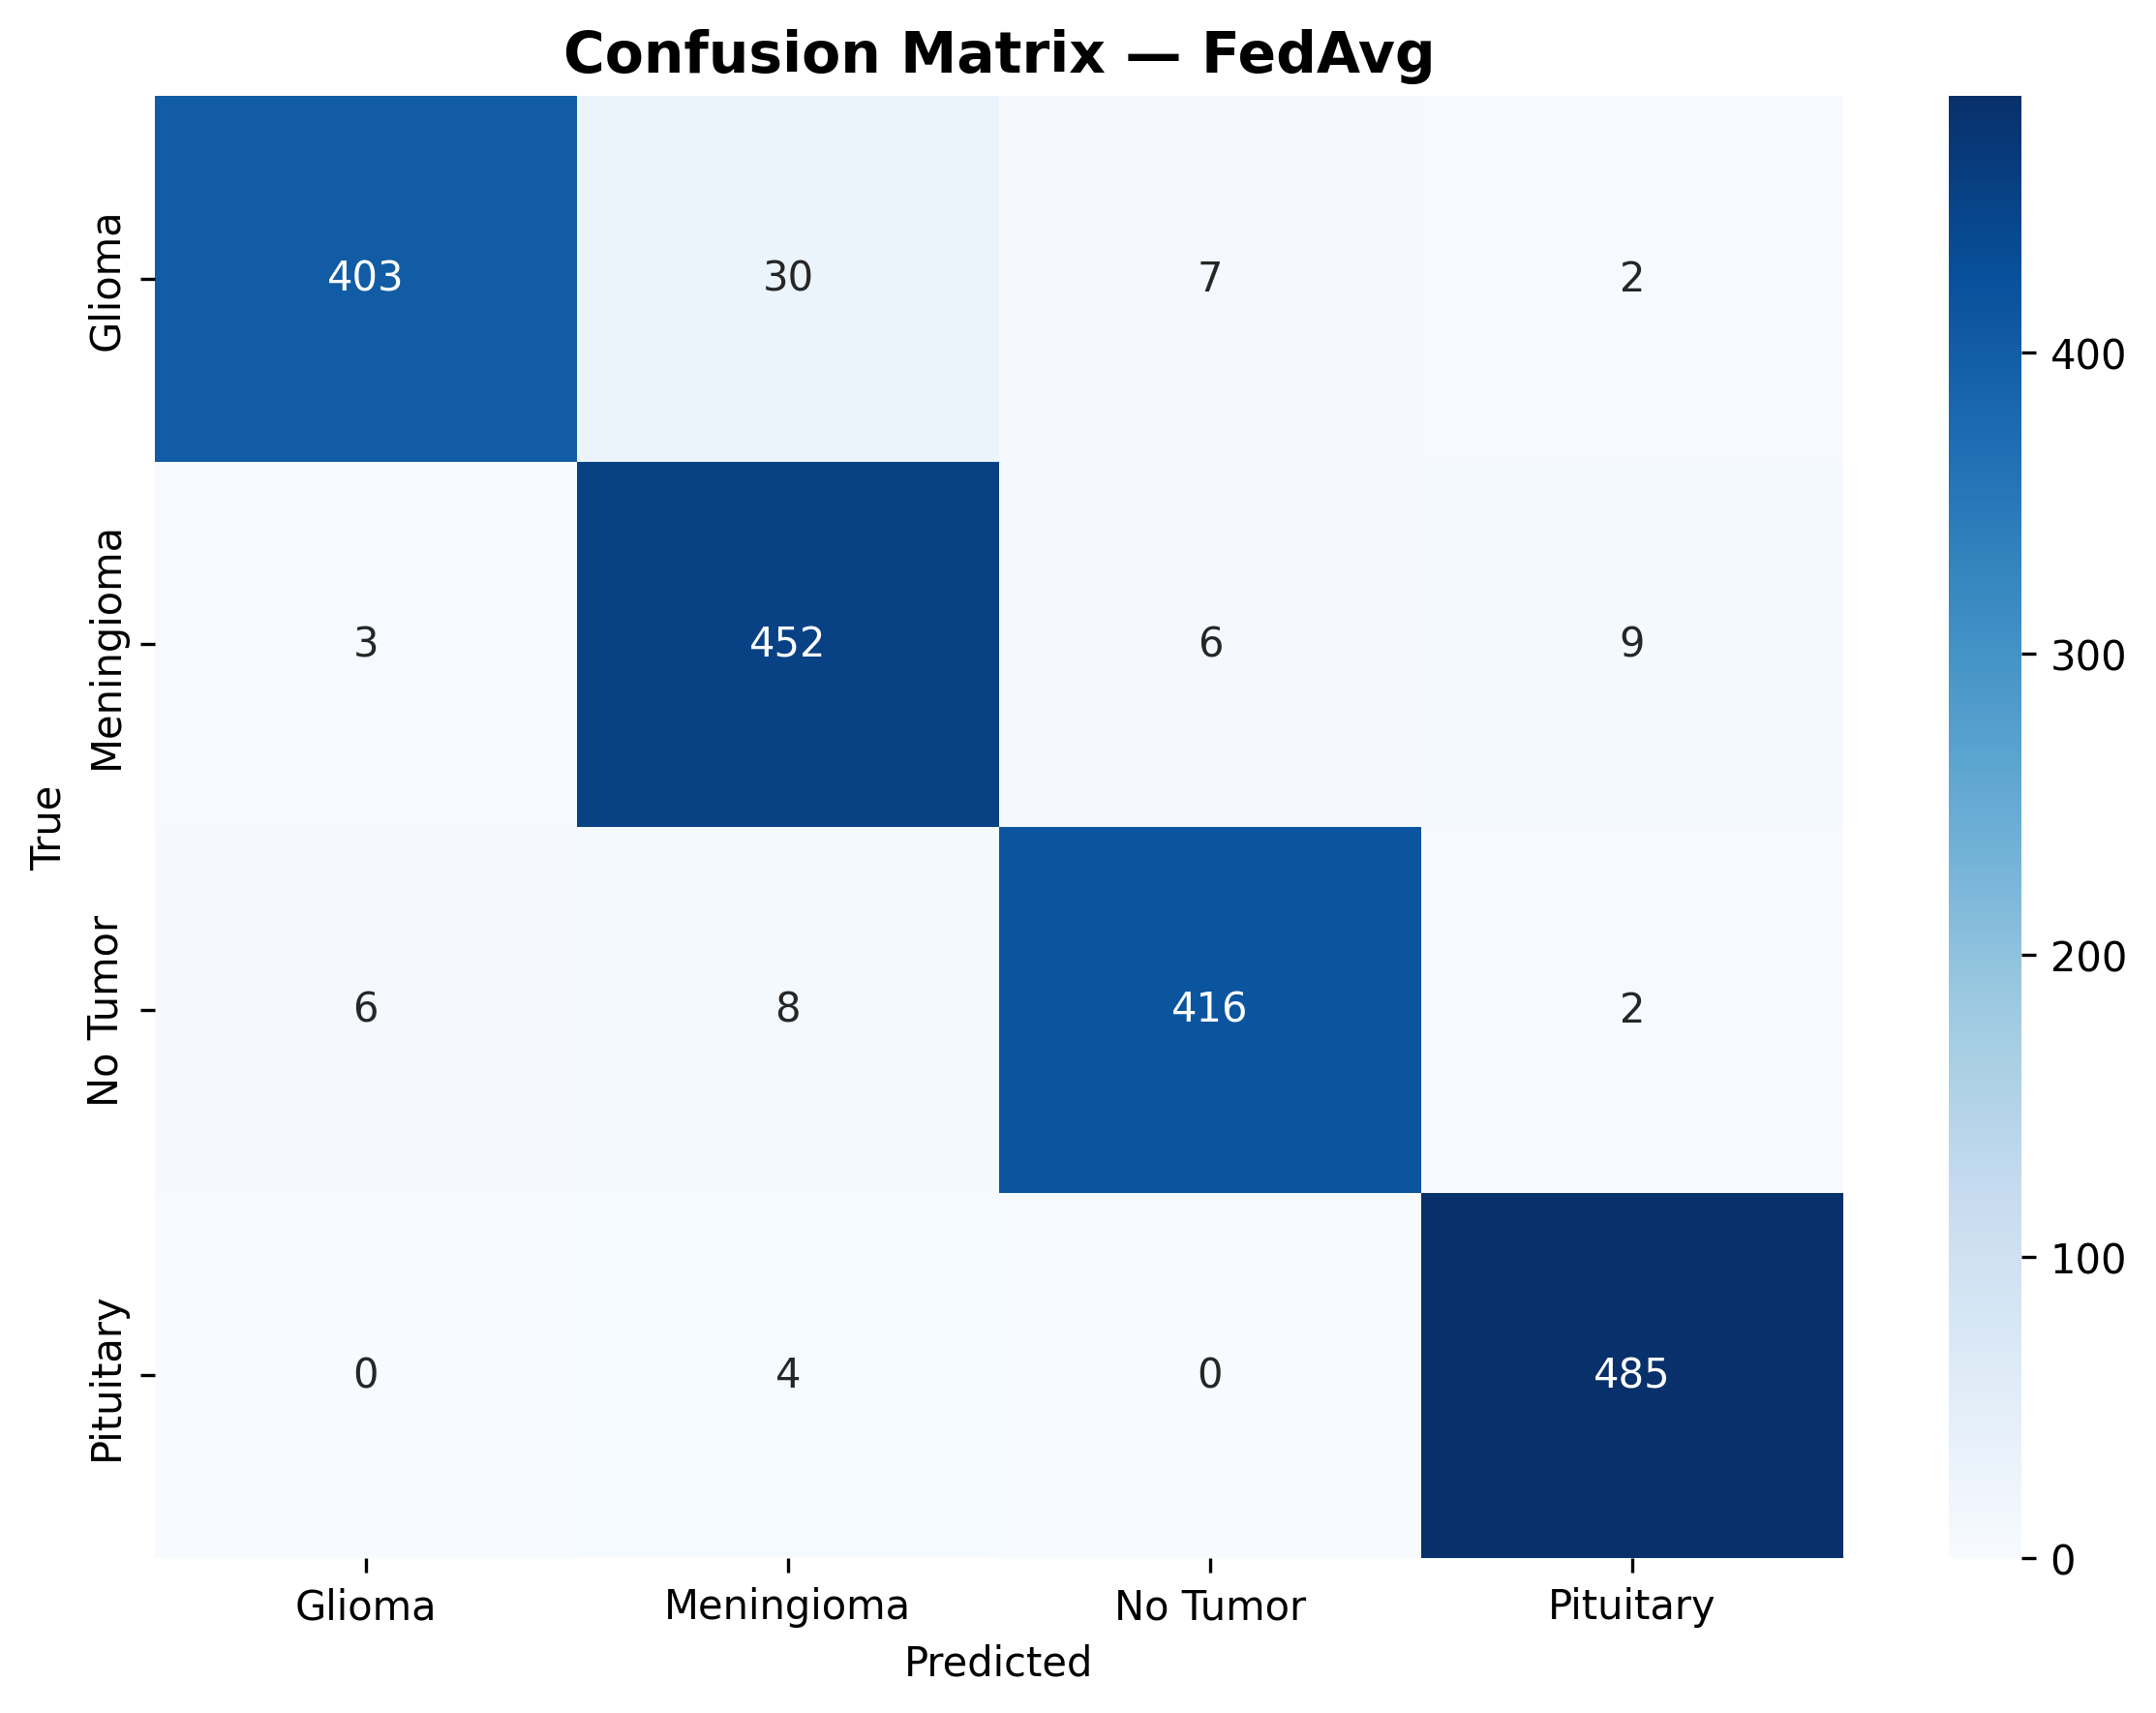
\includegraphics[width=0.48\columnwidth]{s1_cm_fedavg.png}%
  \hfill
  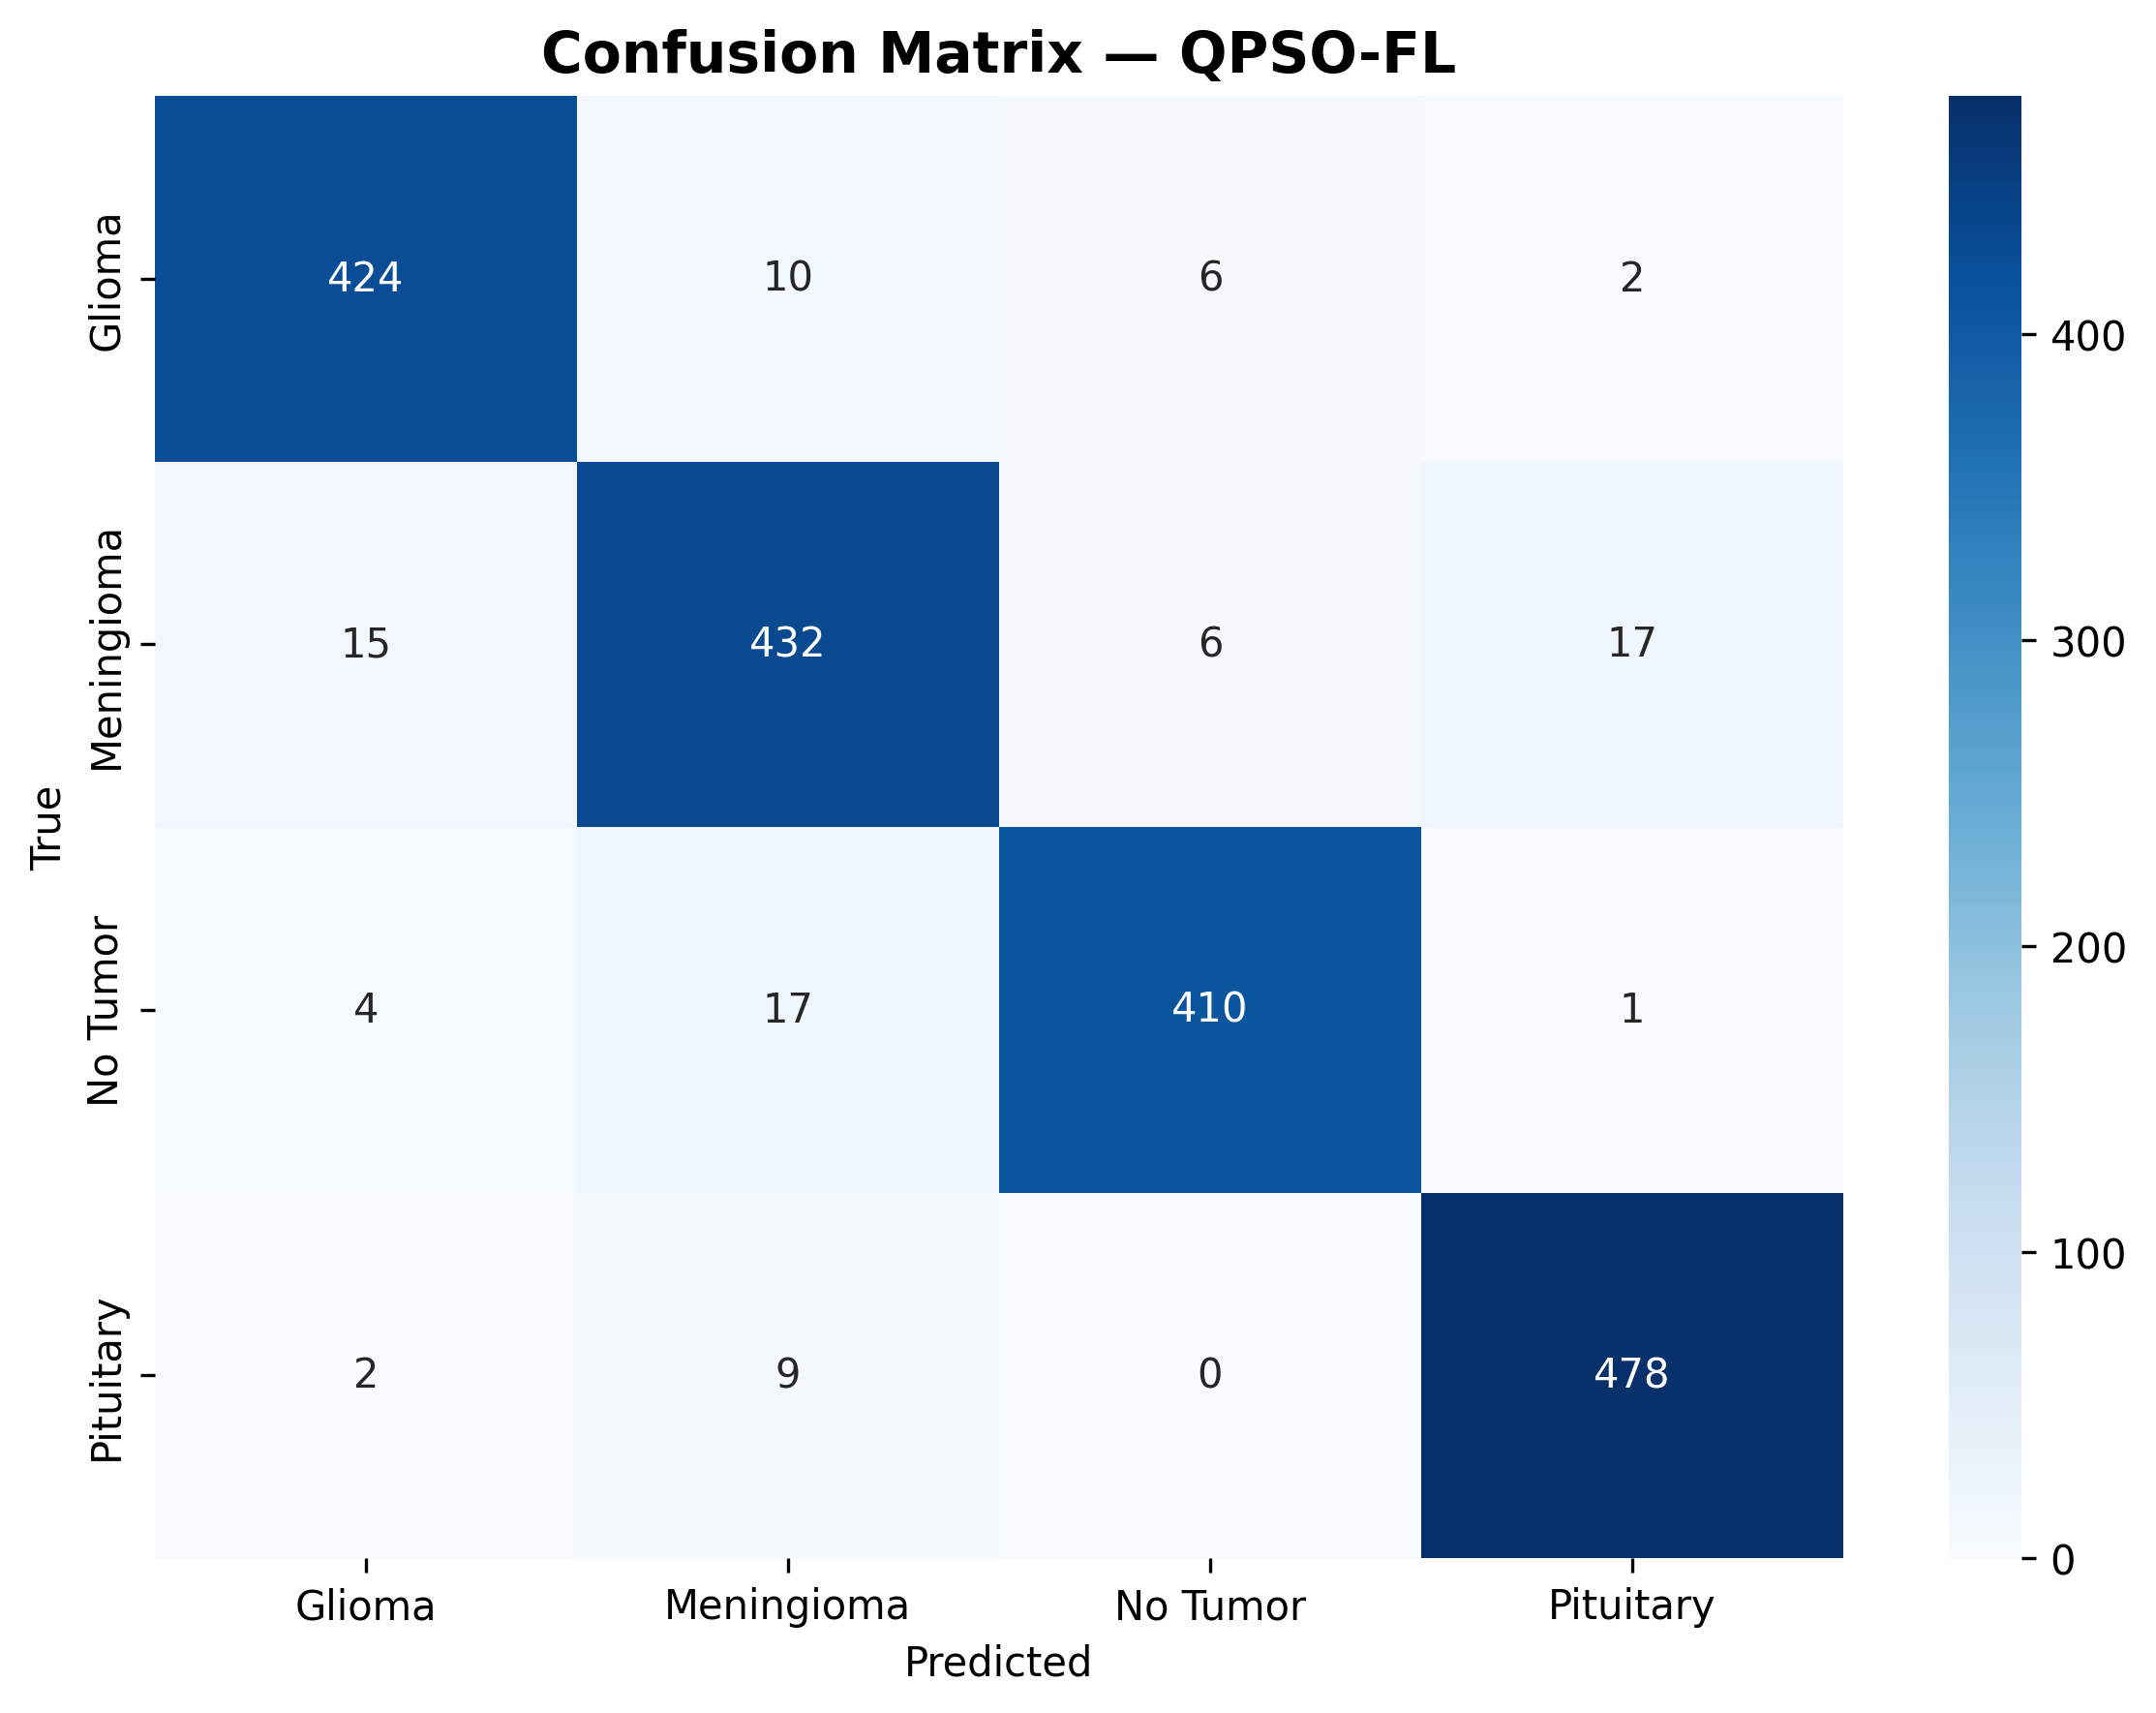
\includegraphics[width=0.48\columnwidth]{s1_cm_qpso.png}}
\caption{Confusion matrices --- Setup~1. Left: FedAvg. Right: FedQPSO.
FedQPSO shows fewer Glioma misclassifications; FedAvg's errors are
concentrated in Glioma--Meningioma confusions.}
\label{fig:cm_s1}
\end{figure}

\begin{figure}[htbp]
\centerline{%
  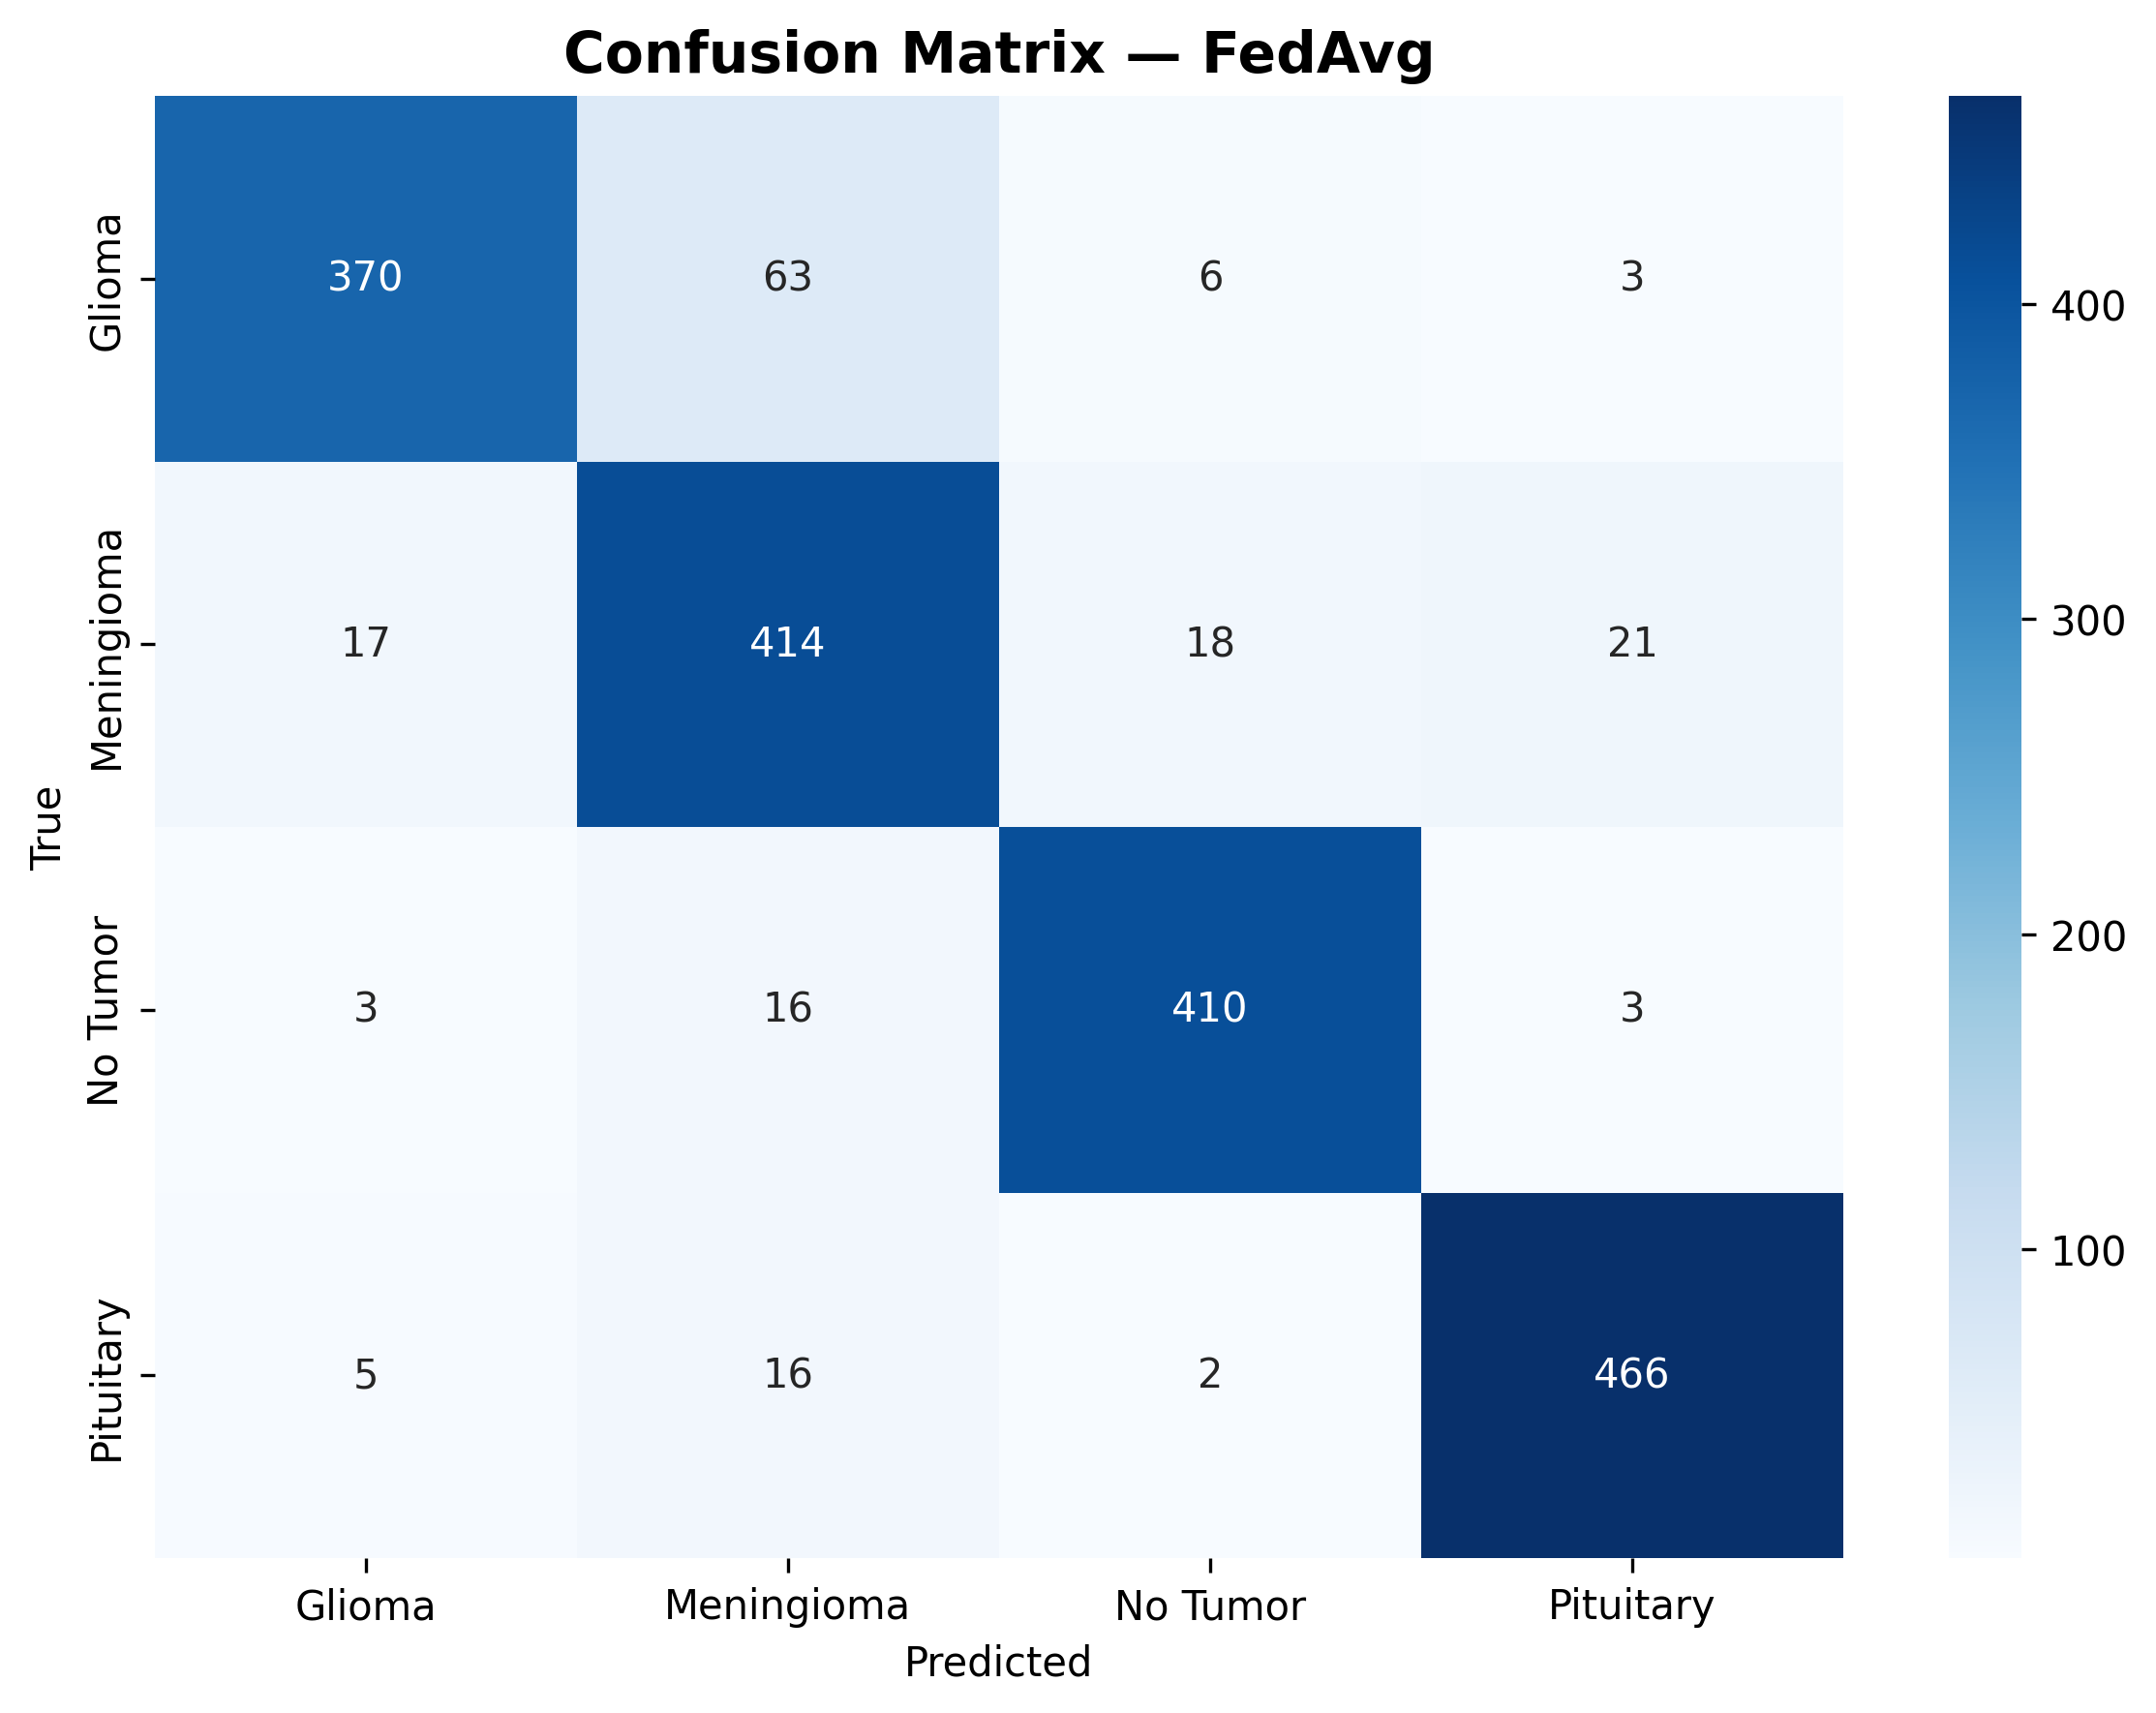
\includegraphics[width=0.48\columnwidth]{s2_cm_fedavg.png}%
  \hfill
  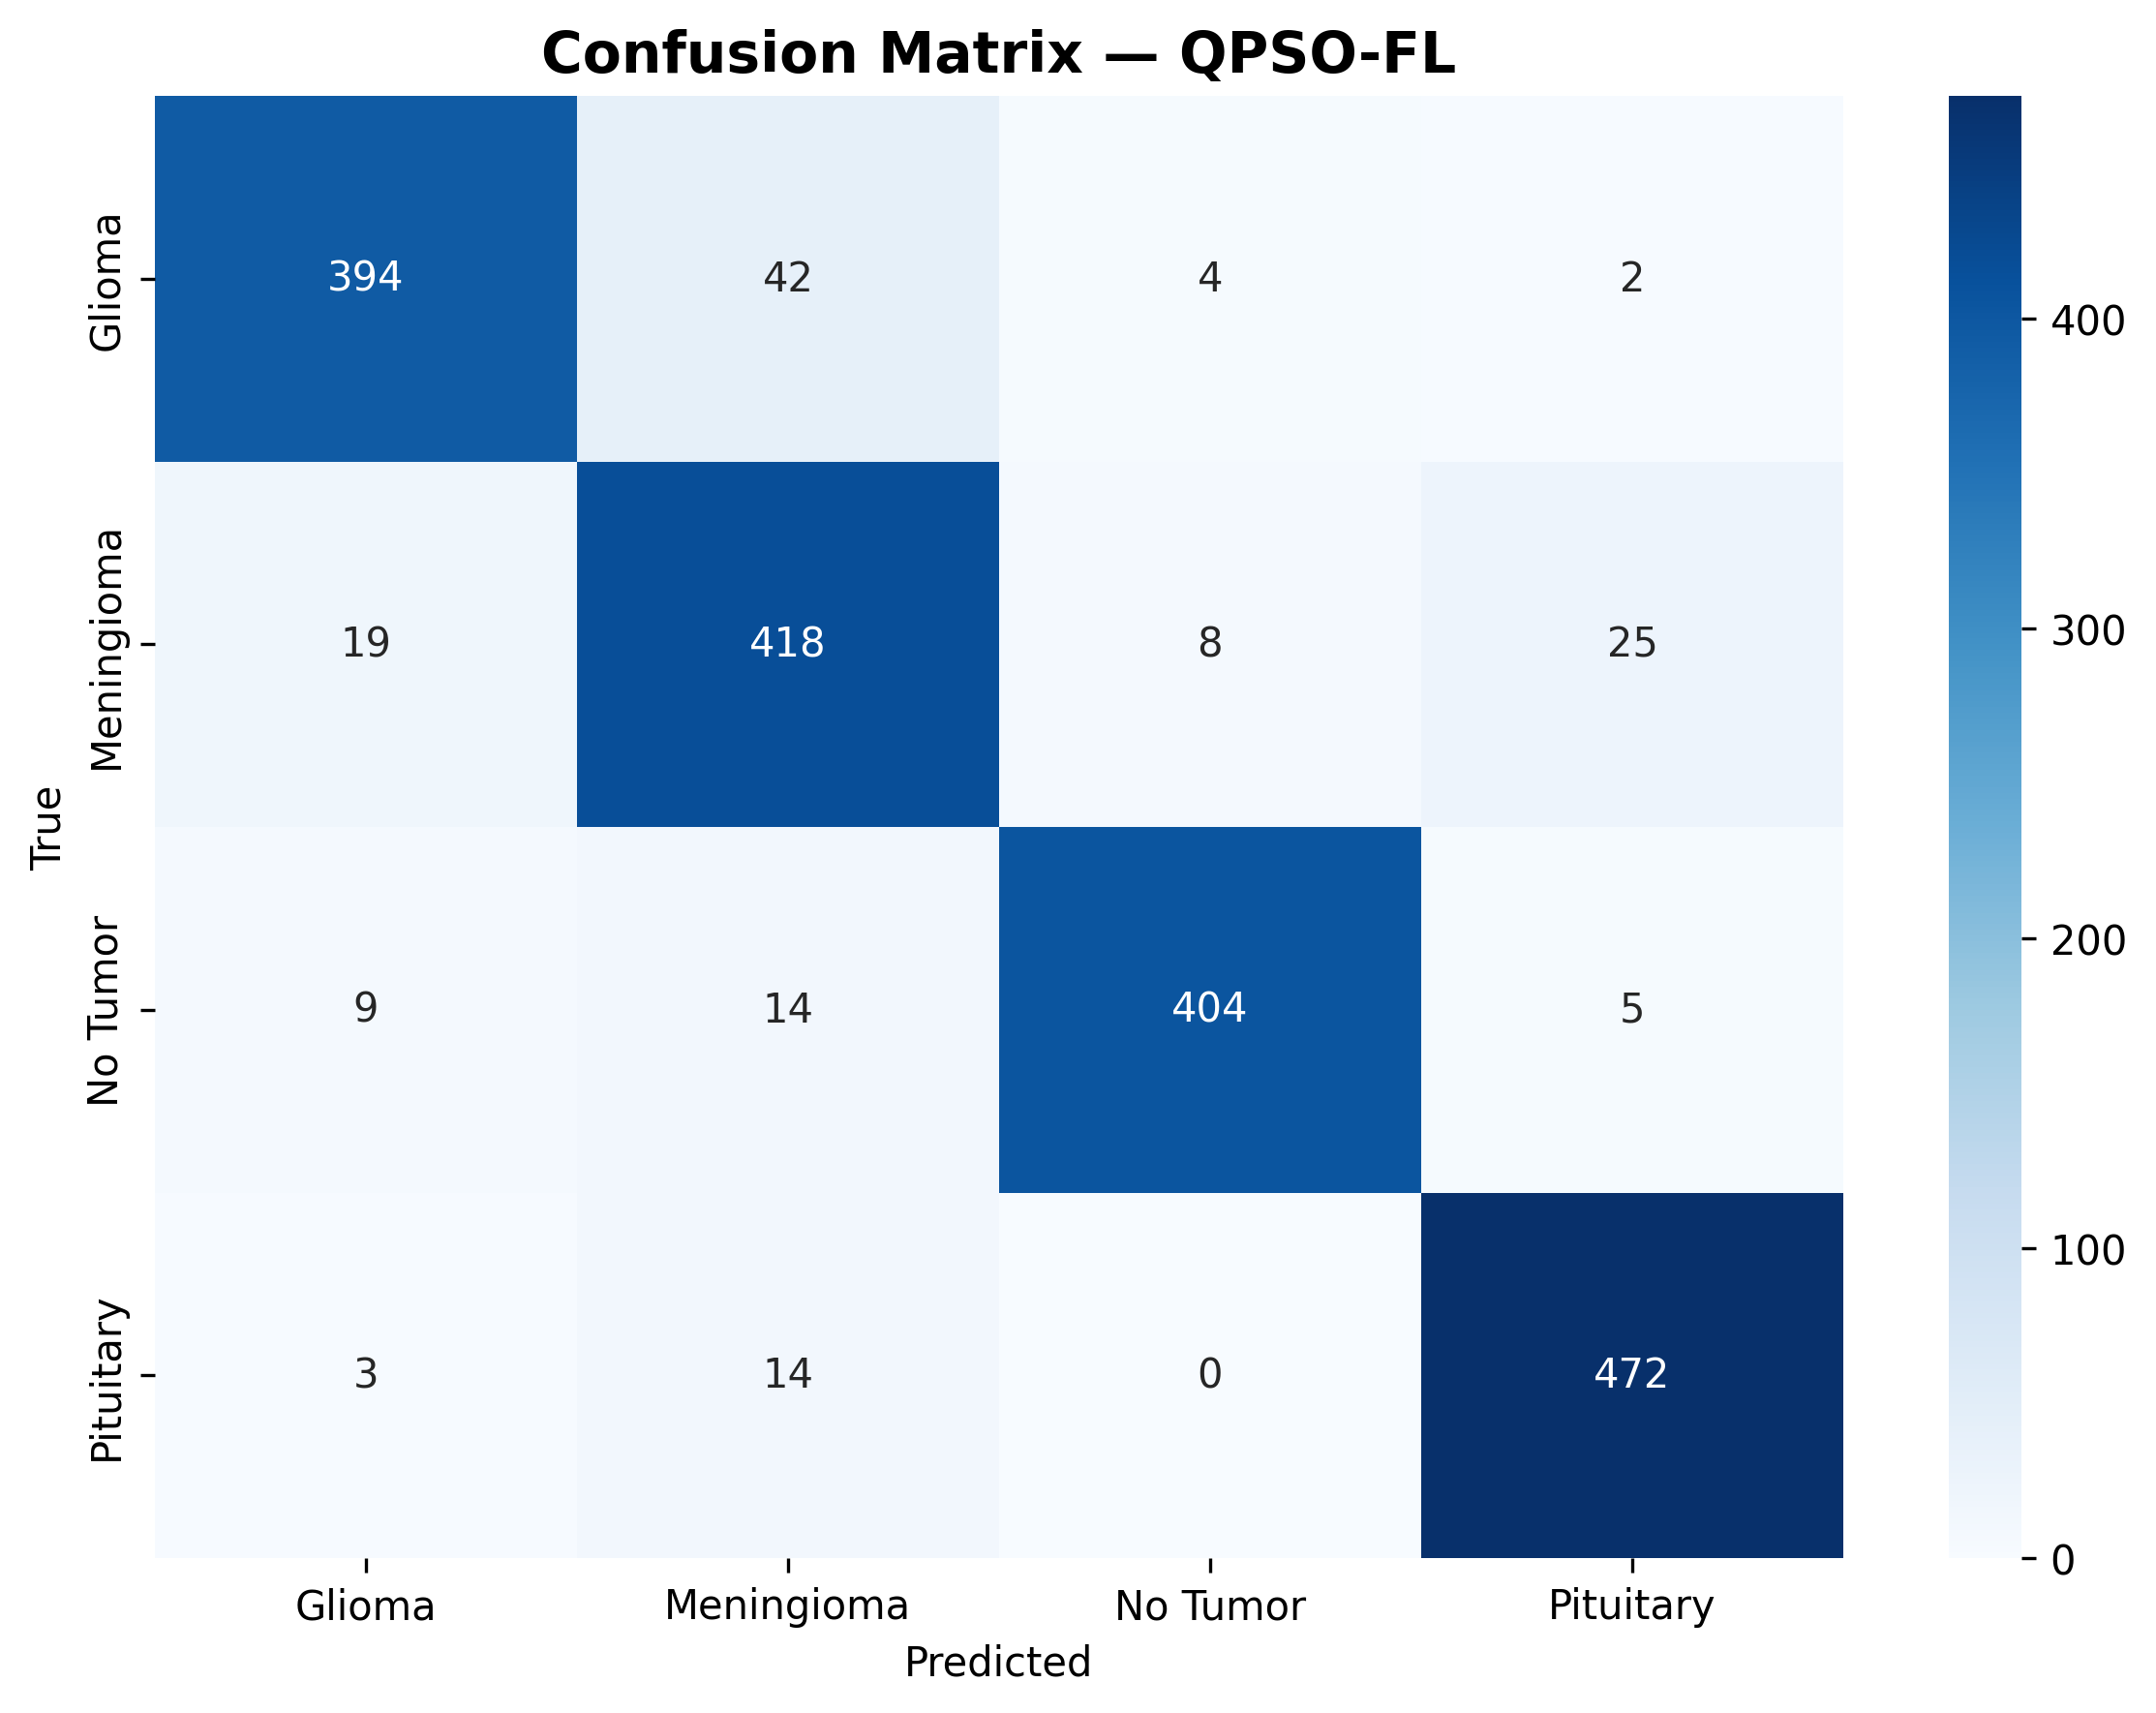
\includegraphics[width=0.48\columnwidth]{s2_cm_qpso.png}}
\caption{Confusion matrices --- Setup~2 (Label Skew). Left: FedAvg.
Right: FedQPSO. Under label skew FedAvg shows pronounced Glioma and
Meningioma off-diagonal errors driven by client distribution bias;
FedQPSO is substantially better-calibrated across all classes.}
\label{fig:cm_s2}
\end{figure}

\subsection{Stability Analysis}

Table~\ref{tab:stability} quantifies accuracy curve stability.

\begin{table}[htbp]
\caption{Accuracy Curve Stability}
\label{tab:stability}
\begin{center}
\begin{tabular}{llcc}
\hline
\textbf{Setup} & \textbf{Metric} & \textbf{FedAvg} & \textbf{FedQPSO}\\
\hline
\multirow{2}{*}{S1}
 & Max round drop (pp)       & $-$11.51 & \textbf{$-$2.45}\\
 & Round-to-round std (pp)   & $\approx$4.0 & \textbf{2.22}\\
\hline
\multirow{2}{*}{S2}
 & Max round drop (pp)       & $-$14.78 & \textbf{$-$3.38}\\
 & Round-to-round std (pp)   & 4.08 & \textbf{2.16}\\
\hline
\end{tabular}
\end{center}
\end{table}

FedQPSO's round-to-round volatility is approximately \textbf{half} that of
FedAvg in both conditions. The maximum accuracy drop across FedQPSO's 200
combined training rounds (3.38\,pp in Setup~2) is less than one-quarter of
FedAvg's largest single-round crash in the easier natural heterogeneity
condition (11.51\,pp). The fitness evaluation step acts as a filter: weight
configurations that destabilize the global model are evaluated against the
validation set and rejected before being committed.

% ============================================================
\section{Discussion}
\label{sec:discussion}
% ============================================================

\subsection{Root Cause of FedAvg's Fairness Failure}
FedAvg's aggregation formula~\eqref{eq:fedavg} assigns weight proportional
to dataset size. Client~3 holds $3.5\times$ more samples than Client~1,
giving it $3.5\times$ more influence over every weight tensor in every
round. This bias is structurally embedded in FedAvg and cannot be mitigated
by adjusting hyperparameters or training duration. Under label skew, the
problem compounds: Client~3's dominant No Tumor class pulls the global model
away from the Glioma-specialized representations needed for Client~1's data.
The result — Client~1 at 60.42\% while the global metric reports 88.16\%
— is not a calibration issue but a structural inequity.

\subsection{How FedQPSO Resolves This}
FedQPSO makes no \emph{a priori} assumption about which client's weights are
``more correct.'' Instead, it proposes, evaluates, and refines candidate
weight configurations against the combined validation set $\mathcal{V}$.
A configuration that achieves low loss for Client~3 but high loss for
Client~1 produces a high aggregate validation loss and is iteratively
replaced. The search converges naturally toward weights satisfying all
clients' objectives simultaneously. This mechanism requires no knowledge
of data distributions, no client reweighting, and no fairness hyperparameter.

\subsection{When FedQPSO Is Most Valuable}
Cohen's $d$ grows from 0.35 (Setup~1) to 1.26 (Setup~2) as heterogeneity
increases. This is the most important finding of the paper: the algorithm
is \emph{self-calibrating} to problem difficulty. When data distributions
are similar (Setup~1), the fitness-guided search produces marginal gains
over FedAvg's weighted mean. When distributions diverge severely (Setup~2),
the fitness evaluation surface becomes sharply differentiated between fair
and unfair weight configurations, and QPSO's global search finds solutions
far outside FedAvg's reach. This means FedQPSO does not require the user
to correctly anticipate heterogeneity severity to be deployed effectively.

\subsection{Clinical Interpretation}
In a deployed federated brain tumor screening network, FedAvg's Setup~2
behavior — 52.92\% Client~1 accuracy at the global accuracy peak — means
that the hospital with the smallest dataset would be screening glioma
patients with a model barely better than random selection. FedQPSO raises
that floor to 80.83\% at the same moment. The 5.43\,pp Glioma recall
improvement translates to approximately 24 additional correct glioma
identifications per 1,000 screened patients — 24 patients who receive
prompt surgical evaluation rather than being misclassified.

\subsection{Computational Trade-offs}
FedQPSO rounds take approximately 75 seconds versus FedAvg's 8 seconds
(9.4$\times$ overhead), borne entirely by the central server. For offline
model development — the typical use case — 125 minutes total training time
is entirely practical. For high-frequency retraining scenarios, overhead
can be reduced by decreasing $T$, applying FedQPSO selectively to
high-variance layers, or interleaving FedAvg and FedQPSO rounds.

% ============================================================
\section{Limitations and Future Work}
\label{sec:limitations}
% ============================================================

\paragraph{Computational cost}
The 9.4$\times$ server overhead limits retraining frequency. Future work
should investigate reducing $T$, selective layer-wise QPSO application,
and periodic FedQPSO scheduling.

\paragraph{Client scale}
Only 3 clients were evaluated. Validation with 5--10 clients at varying
institutional sizes would strengthen generalizability claims.

\paragraph{Architecture}
SimpleCNN's deliberate simplicity isolates aggregation performance.
Future work should evaluate FedQPSO with deeper architectures
(EfficientNet-B0, ResNet-18) and appropriate ablation controls.

\paragraph{Hyperparameter sensitivity}
$\beta = 0.6$ and $T = 5$ were adopted from the MNIST pilot
\cite{edla2025mnist} without task-specific tuning. Sensitivity analyses
and adaptive $\beta$ scheduling may improve performance further.

\paragraph{Single seed}
Run-to-run variance across multiple random seeds was not measured.
Future work should report confidence intervals over at least 3 runs.

\paragraph{Privacy guarantees}
Structural FL privacy is provided. Adding differential privacy
guarantees would complement FedQPSO's fairness benefits.

% ============================================================
\section{Conclusion}
\label{sec:conclusion}
% ============================================================

We introduced \textbf{FedQPSO}, a server-side federated aggregation algorithm
that replaces FedAvg's dataset-weighted mean with a layer-by-layer Quantum
Particle Swarm Optimization search guided by combined cross-client validation
loss. Applied to four-class brain tumor MRI classification across three
heterogeneous simulated clinical sites, FedQPSO consistently and significantly
outperforms FedAvg across every fairness and stability metric:

\begin{itemize}
    \item FedQPSO reduces FedAvg's max-min inter-client accuracy gap by
    \textbf{81\%} under natural heterogeneity and \textbf{72\%} under
    label skew.

    \item FedQPSO is the only method maintaining $\geq$80\% accuracy at
    the weakest client under label skew — a direct patient safety benefit.

    \item FedQPSO achieves the highest Glioma recall in both experimental
    conditions (0.9593; 0.8914) and the most stable accuracy trajectories
    (max drop 3.38\,pp vs.\ 14.78\,pp for FedAvg).

    \item FedQPSO statistically significantly outperforms FedAvg in both
    setups, with Cohen's $d$ scaling from 0.35 to 1.26 as heterogeneity
    increases — confirming the algorithm is most advantageous precisely
    when the clinical stakes are highest.

    \item The fairness benefit emerges from a simple implicit mechanism
    — combined cross-client validation fitness evaluation — requiring no
    explicit fairness objective, reweighting, or hyperparameter tuning.
\end{itemize}

FedQPSO establishes that weighted averaging is not the only, nor the best,
approach to federated aggregation under Non-IID conditions. It offers a
practical, deployable alternative that closes the performance gap between
the best-served and worst-served institutions in federated medical imaging
networks.

% ============================================================
\section*{Acknowledgment}
The authors acknowledge the support of the Department of Computer Science \&
Engineering, Matrusri Engineering College. Compute resources were provided
via Kaggle's GPU platform (Tesla P100-16GB). The Masoud Brain Tumor MRI
dataset and the BRISC 2025 dataset, both publicly available on Kaggle, are
gratefully acknowledged.

% ============================================================
\begin{thebibliography}{00}

\bibitem{mcmahan2017}
H.~B. McMahan, E.~Moore, D.~Ramage, S.~Hampson, and B.~A. y~Arcas,
``Communication-efficient learning of deep networks from decentralized data,''
in \textit{Proc.\ 20th Int.\ Conf.\ Artif.\ Intell.\ Stat.\ (AISTATS)},
Fort Lauderdale, FL, USA, Apr.\ 2017, pp.~1273--1282.

\bibitem{zhao2018}
J.~Zhao, M.~Li, J.~Xu, and W.~Li,
``Federated learning with non-IID data,''
\textit{arXiv:1806.00582}, Jun.\ 2018.

\bibitem{sun2004qpso}
J.~Sun, B.~Feng, and W.~Xu,
``Particle swarm optimization with particles having quantum behavior,''
in \textit{Proc.\ 2004 Congr.\ Evol.\ Comput.\ (CEC)}, Portland, OR, USA,
Jun.\ 2004, vol.~1, pp.~325--331.

\bibitem{sheller2018}
M.~J. Sheller, G.~A. Reina, B.~Edwards, J.~Martin, and S.~Bakas,
``Multi-institutional deep learning modeling without sharing patient data:
A feasibility study on brain tumor segmentation,''
in \textit{Proc.\ Int.\ MICCAI Brainlesion Workshop}, Granada, Spain,
Sep.\ 2018, pp.~92--104.

\bibitem{rieke2020}
N.~Rieke \textit{et al.},
``The future of digital health with federated learning,''
\textit{npj Digit.\ Med.}, vol.~3, no.~1, pp.~1--7, Sep.\ 2020.

\bibitem{sultan2019}
H.~H. Sultan, N.~M. Salem, and W.~Al-Atabany,
``Multi-classification of brain tumor images using deep neural network,''
\textit{IEEE Access}, vol.~7, pp.~69\,215--69\,225, 2019.

\bibitem{ostrom2021}
Q.~T. Ostrom \textit{et al.},
``CBTRUS statistical report: Primary brain and other central nervous system
tumors diagnosed in the United States in 2014--2018,''
\textit{Neuro-oncology}, vol.~23, no.~suppl\_3, pp.~iii1--iii105, 2021.

\bibitem{hipaa}
U.S.\ Department of Health \& Human Services,
``Health Insurance Portability and Accountability Act (HIPAA) of 1996,''
Public Law 104-191, 1996.

\bibitem{kennedy1995}
J.~Kennedy and R.~Eberhart,
``Particle swarm optimization,''
in \textit{Proc.\ ICNN'95 --- Int.\ Conf.\ Neural Netw.}, Perth, WA,
Australia, Nov.--Dec.\ 1995, vol.~4, pp.~1942--1948.

\bibitem{fedpso2021}
J.~Park, H.~J. Kim, and J.~Moon,
``FedPSO: Federated learning using particle swarm optimization to
reduce communication costs,''
\textit{Sensors}, vol.~21, no.~2, p.~600, Jan.\ 2021.

\bibitem{li2021survey}
T.~Li, A.~K. Sahu, A.~Talwalkar, and V.~Smith,
``Federated learning: Challenges, methods, and future directions,''
\textit{IEEE Signal Process.\ Mag.}, vol.~37, no.~3, pp.~50--60,
May 2020.

\bibitem{masoud}
M.~Nickparvar,
``Brain tumor MRI dataset,''
Kaggle, 2021. [Online]. Available:
\url{https://www.kaggle.com/datasets/masoudnickparvar/brain-tumor-mri-dataset}

\bibitem{brisc}
BRISC Dataset Contributors,
``BRISC 2025 brain tumor classification dataset,''
Kaggle, 2025. [Online]. Available:
\url{https://www.kaggle.com/datasets/briscdataset/}

\bibitem{edla2025mnist}
D.~T. Edla,
``Enhancing federated learning with quantum-inspired particle swarm
optimization: An {IID} {MNIST} study,'' (Paper ID: CSE-104)
in \textit{Proc.\ AICTE Sponsored Natl.\ Conf.\ Innovations, Challenges
and Solutions in Eng., Sci.\ and Technol.\ (NCICSET'25)},
Sri Indu College of Engineering and Technology, Hyderabad, India,
Dec.\ 17--18, 2025.

\end{thebibliography}

\end{document}